\documentclass[12pt]{article}

\usepackage[a4paper,margin=2cm]{geometry}

\usepackage{amsmath}
\usepackage{amssymb}
\usepackage{mathtools}
\usepackage{dsfont}

\usepackage{listings}

\usepackage{booktabs} % For tables
\usepackage[table,xcdraw]{xcolor} % For tables

\usepackage{svg} % for .svg's

\usepackage{parskip}

\usepackage{tikz} % TikZ

\usepackage{enumerate}
\usepackage{enumitem}

\usepackage{nameref}

\usepackage{xcolor}

\usepackage{subfiles}

\usepackage{verbatim}

\definecolor{codegreen}{rgb}{0,0.6,0}
\definecolor{codegray}{rgb}{0.5,0.5,0.5}
\definecolor{codepurple}{rgb}{0.58,0,0.82}
\definecolor{backcolour}{rgb}{0.95,0.95,0.92}

\lstdefinestyle{mystyle}{
    backgroundcolor=\color{backcolour},
    commentstyle=\color{codegreen},
    keywordstyle=\color{magenta},
    numberstyle=\tiny\color{codegray},
    stringstyle=\color{codepurple},
    basicstyle=\ttfamily\footnotesize,
    breakatwhitespace=false,
    breaklines=true,
    captionpos=b,
    keepspaces=true,
    numbers=left,
    numbersep=5pt,
    showspaces=false,
    showstringspaces=false,
    showtabs=false,
    tabsize=2
}

\lstset{style=mystyle}

\DeclarePairedDelimiter\abs{\lvert}{\rvert}
\DeclarePairedDelimiter\Abs{\lVert}{\rVert}

\usepackage{fancyhdr}

\pagestyle{fancy}
\lhead{\today}
\chead{Exercise 5\\Machine Learning}
\rhead{Til Mohr\\Simon Michau\\Marc Ludevid Wulf}

\setlength{\headheight}{50pt}

\begin{document}

\section*{Question 1}
\subsection*{(a)}
Number of SV: 3\\
Accuracy on train data with C = 1000: 1.0 \\
Accuracy on test data with C = 1000: 0.8648648648648649 \\

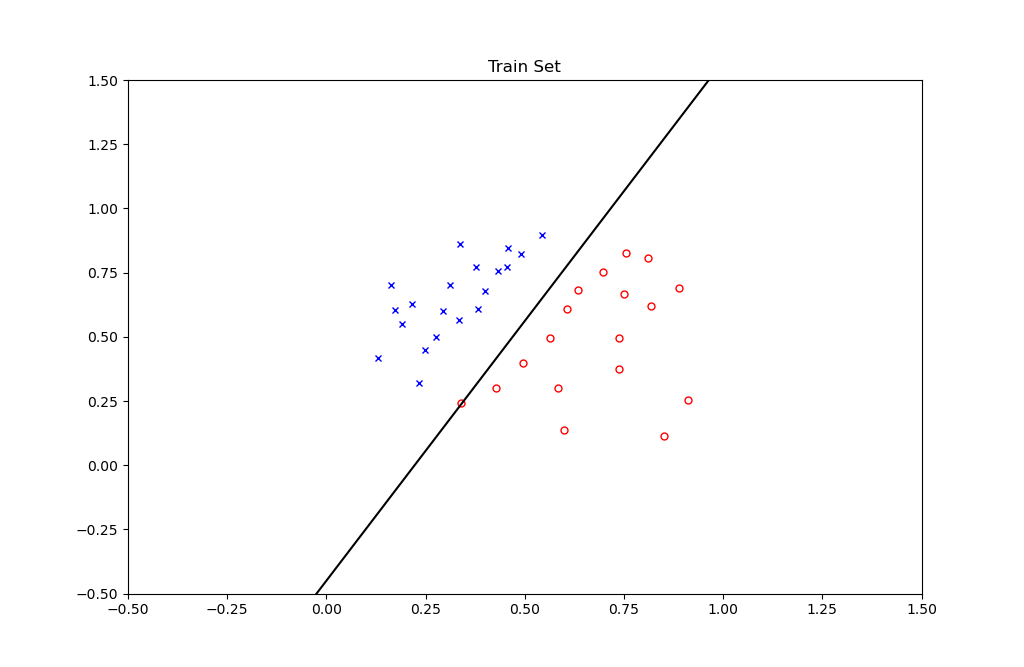
\includegraphics[width=.5\textwidth]{q1_svm_python/Figure_1.png}
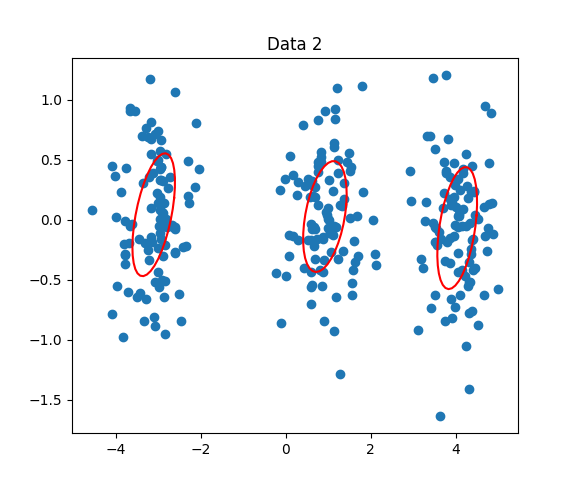
\includegraphics[width=.5\textwidth]{q1_svm_python/Figure_2.png}

\subsubsection*{Adjustments to \texttt{apply\_a.py}}
\texttt{python apply\_a.py} threw a lot of errors, which were mainly due to not enforcing a datatype (i.e. matrix vs nparray) and not taking the dimensions requested in \texttt{simlin.py} into account.\\

For this reason, we have modified \texttt{apply\_a.py}.

\subsection*{(b+c)}
\subsubsection*{1-vs-3}
Number of SV: 26 \\
Width of margin: 0.000527852066940575 \\
Train Error 1-vs-3: 7 \\
Test Error 1-vs-3: 0.013953488372093023 \\

\subsubsection*{3-vs-8}
Number of SV: 89 \\
Width of margin: 0.00010191438464165348 \\
Train Error 3-vs-8:  66 \\
Test Error 3-vs-8:  0.09939759036144578

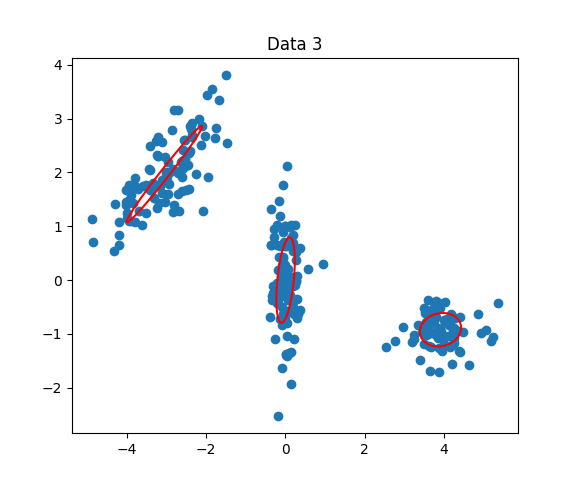
\includegraphics[width=.5\textwidth]{q1_svm_python/Figure_3.png}
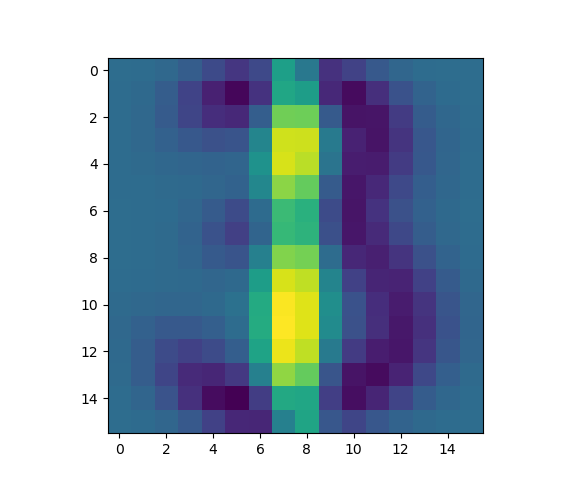
\includegraphics[width=.5\textwidth]{q1_svm_python/Figure_4.png}
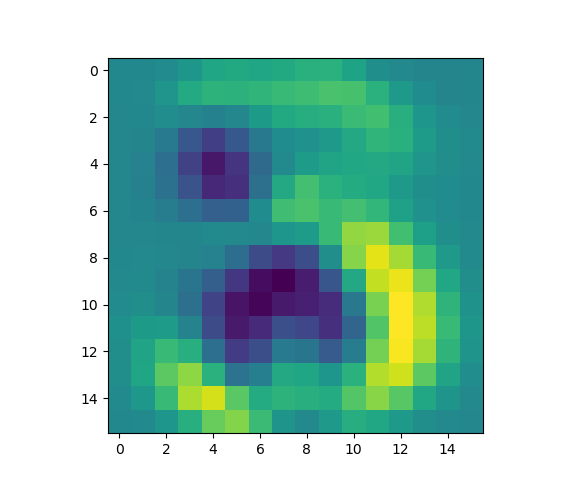
\includegraphics[width=.5\textwidth]{q1_svm_python/Figure_5.png}


\subsubsection*{Adjustments to \texttt{apply\_bc.py}}
As \texttt{python apply\_a.py}, \texttt{python apply\_bc.py} threw a lot of errors, which were mainly due to not enforcing a datatype (i.e. matrix vs nparray) and not taking the dimensions requested in \texttt{simlin.py} into account.\\

For this reason, we have modified \texttt{apply\_bc.py}.

\subsection*{(d)}
Accuracy of kernel SVM with C=1000 and norm=5: 0.40540540540540543

This shows, that the accuracy of the kernel SVM is much lower than the accuracy of the linear SVM.

\subsubsection*{Adjustments to \texttt{apply\_d.py} and \texttt{svmkern.py}}
There was a mismatch between the number of variables unpacked from the function \texttt{svmkern} in \texttt{apply\_d.py} and the number of variables to be returned by this function, defined by its description. We have extended the function to return the same values as \texttt{svmlin}.\\
As with the previous adjustments that had to be made, we again had to enforce datatypes and dimensions.
\newpage
\section*{Question 1}
\subsection*{(a)}
Number of SV: 3\\
Accuracy on train data with C = 1000: 1.0 \\
Accuracy on test data with C = 1000: 0.8648648648648649 \\

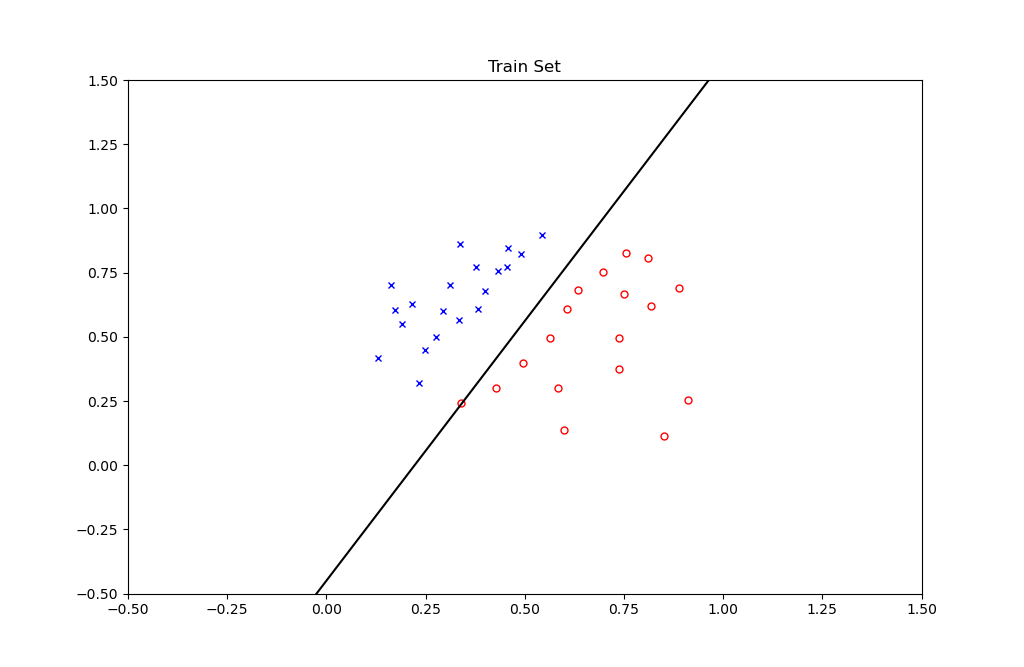
\includegraphics[width=.5\textwidth]{q1_svm_python/Figure_1.png}
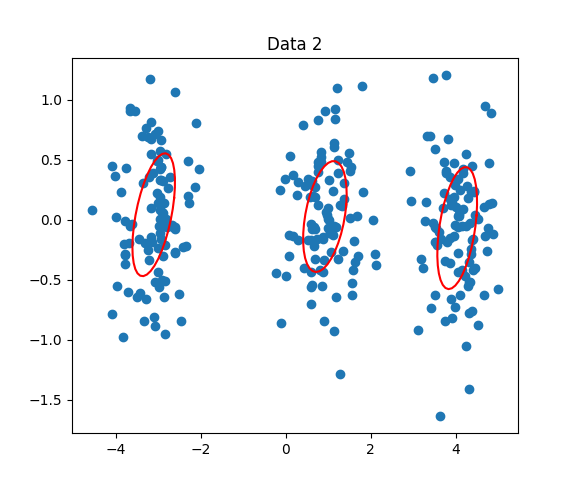
\includegraphics[width=.5\textwidth]{q1_svm_python/Figure_2.png}

\subsubsection*{Adjustments to \texttt{apply\_a.py}}
\texttt{python apply\_a.py} threw a lot of errors, which were mainly due to not enforcing a datatype (i.e. matrix vs nparray) and not taking the dimensions requested in \texttt{simlin.py} into account.\\

For this reason, we have modified \texttt{apply\_a.py}.

\subsection*{(b+c)}
\subsubsection*{1-vs-3}
Number of SV: 26 \\
Width of margin: 0.000527852066940575 \\
Train Error 1-vs-3: 7 \\
Test Error 1-vs-3: 0.013953488372093023 \\

\subsubsection*{3-vs-8}
Number of SV: 89 \\
Width of margin: 0.00010191438464165348 \\
Train Error 3-vs-8:  66 \\
Test Error 3-vs-8:  0.09939759036144578

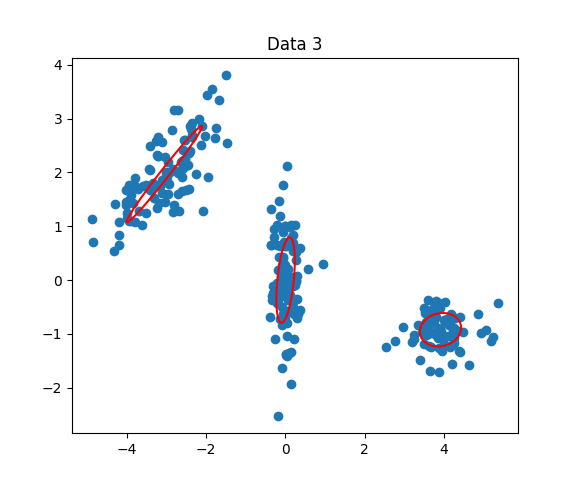
\includegraphics[width=.5\textwidth]{q1_svm_python/Figure_3.png}
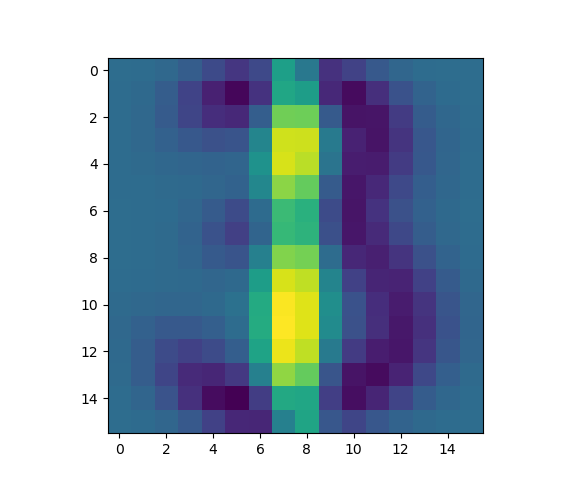
\includegraphics[width=.5\textwidth]{q1_svm_python/Figure_4.png}
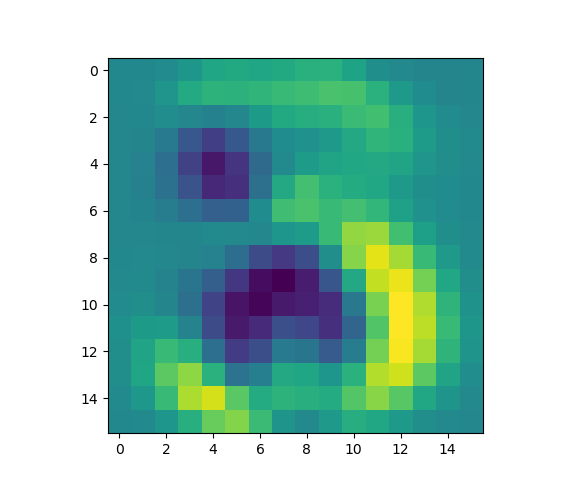
\includegraphics[width=.5\textwidth]{q1_svm_python/Figure_5.png}


\subsubsection*{Adjustments to \texttt{apply\_bc.py}}
As \texttt{python apply\_a.py}, \texttt{python apply\_bc.py} threw a lot of errors, which were mainly due to not enforcing a datatype (i.e. matrix vs nparray) and not taking the dimensions requested in \texttt{simlin.py} into account.\\

For this reason, we have modified \texttt{apply\_bc.py}.

\subsection*{(d)}
Accuracy of kernel SVM with C=1000 and norm=5: 0.40540540540540543

This shows, that the accuracy of the kernel SVM is much lower than the accuracy of the linear SVM.

\subsubsection*{Adjustments to \texttt{apply\_d.py} and \texttt{svmkern.py}}
There was a mismatch between the number of variables unpacked from the function \texttt{svmkern} in \texttt{apply\_d.py} and the number of variables to be returned by this function, defined by its description. We have extended the function to return the same values as \texttt{svmlin}.\\
As with the previous adjustments that had to be made, we again had to enforce datatypes and dimensions.
\newpage
\section*{Question 1}
\subsection*{(a)}
Number of SV: 3\\
Accuracy on train data with C = 1000: 1.0 \\
Accuracy on test data with C = 1000: 0.8648648648648649 \\

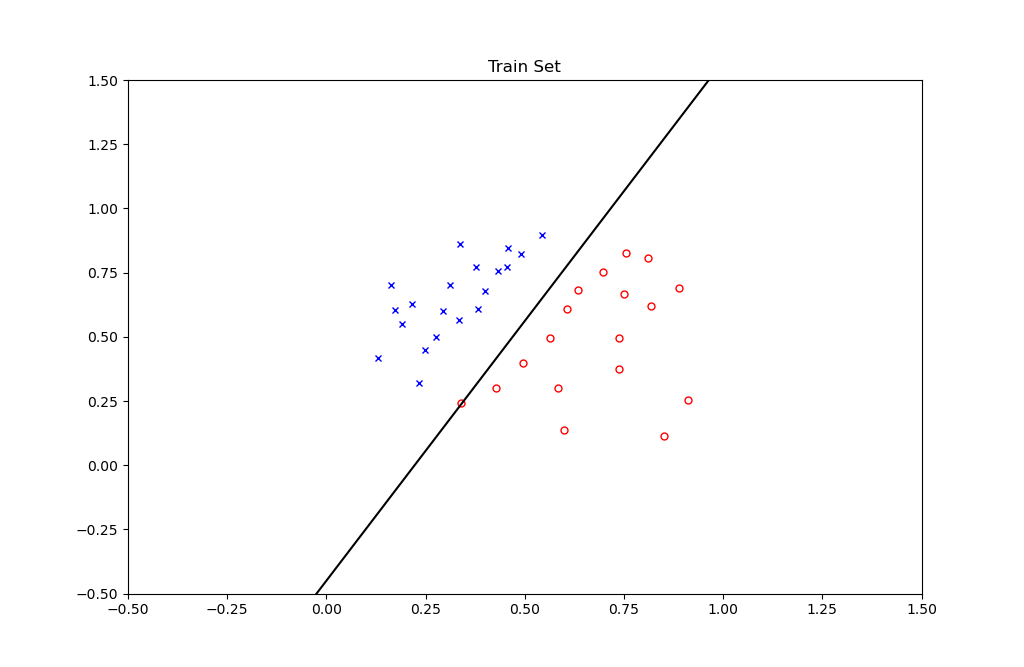
\includegraphics[width=.5\textwidth]{q1_svm_python/Figure_1.png}
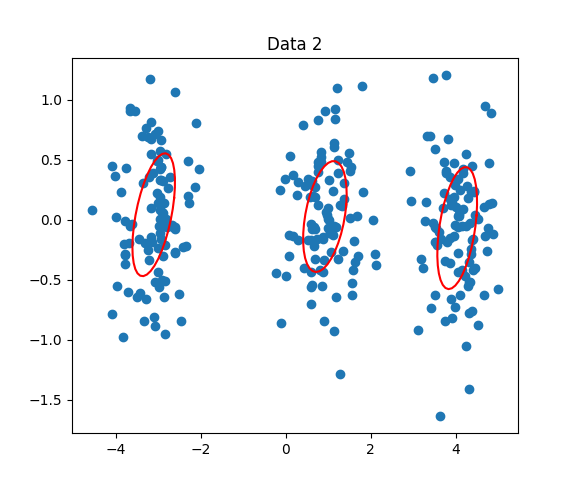
\includegraphics[width=.5\textwidth]{q1_svm_python/Figure_2.png}

\subsubsection*{Adjustments to \texttt{apply\_a.py}}
\texttt{python apply\_a.py} threw a lot of errors, which were mainly due to not enforcing a datatype (i.e. matrix vs nparray) and not taking the dimensions requested in \texttt{simlin.py} into account.\\

For this reason, we have modified \texttt{apply\_a.py}.

\subsection*{(b+c)}
\subsubsection*{1-vs-3}
Number of SV: 26 \\
Width of margin: 0.000527852066940575 \\
Train Error 1-vs-3: 7 \\
Test Error 1-vs-3: 0.013953488372093023 \\

\subsubsection*{3-vs-8}
Number of SV: 89 \\
Width of margin: 0.00010191438464165348 \\
Train Error 3-vs-8:  66 \\
Test Error 3-vs-8:  0.09939759036144578

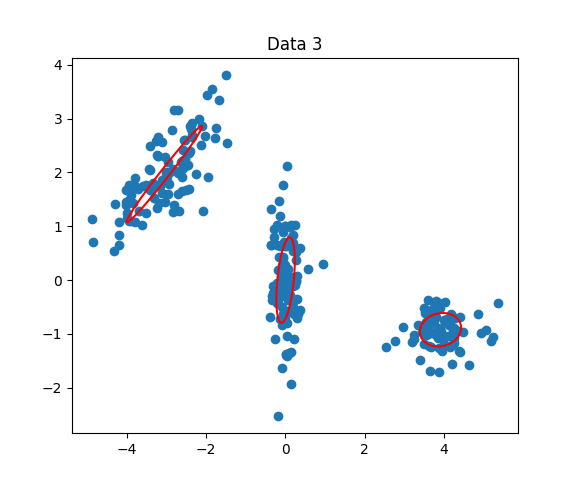
\includegraphics[width=.5\textwidth]{q1_svm_python/Figure_3.png}
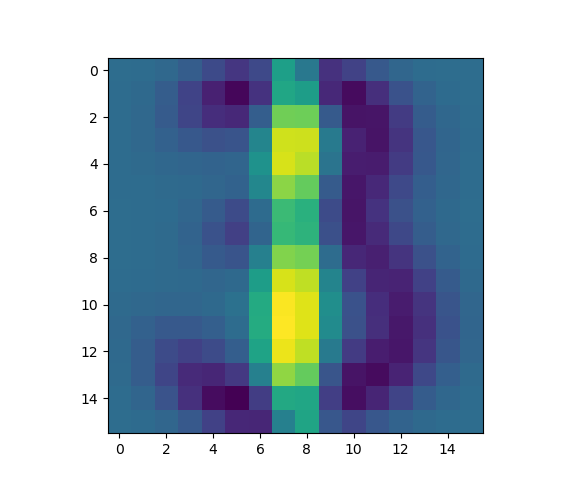
\includegraphics[width=.5\textwidth]{q1_svm_python/Figure_4.png}
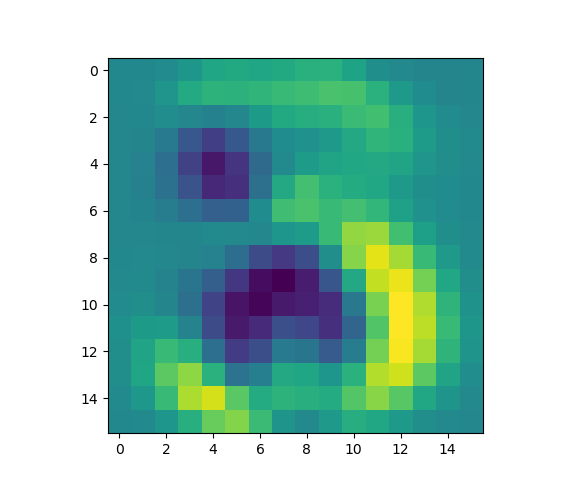
\includegraphics[width=.5\textwidth]{q1_svm_python/Figure_5.png}


\subsubsection*{Adjustments to \texttt{apply\_bc.py}}
As \texttt{python apply\_a.py}, \texttt{python apply\_bc.py} threw a lot of errors, which were mainly due to not enforcing a datatype (i.e. matrix vs nparray) and not taking the dimensions requested in \texttt{simlin.py} into account.\\

For this reason, we have modified \texttt{apply\_bc.py}.

\subsection*{(d)}
Accuracy of kernel SVM with C=1000 and norm=5: 0.40540540540540543

This shows, that the accuracy of the kernel SVM is much lower than the accuracy of the linear SVM.

\subsubsection*{Adjustments to \texttt{apply\_d.py} and \texttt{svmkern.py}}
There was a mismatch between the number of variables unpacked from the function \texttt{svmkern} in \texttt{apply\_d.py} and the number of variables to be returned by this function, defined by its description. We have extended the function to return the same values as \texttt{svmlin}.\\
As with the previous adjustments that had to be made, we again had to enforce datatypes and dimensions.

\end{document}